\chapter{Empirical Evaluation.}

\section{Introduction.}

To conduct an empirical study one needs means to compare different algorithms. Traditional multi-objective optimization have repositories of data sets, with each data set describing a particular problem. These data sets allow us to identify weaknesses or advantages of different algorithms. They also allow us to make a cross-comparison between different algorithms.\\

Reinforcement learning in general and multi-objective reinforcement learning in particular are very different from traditional multi-objective optimization. Reinforcement learning is a multi-step decision making process with a number of actions available at each state at every time step. Add to this a factor of randomness associated with state transition and reward functions. Having all these factors substantially complicates the creation of a test problem. Unlike the general multi-objective optimization, in reinforcement learning a test problem is not a static data set but rather a software which reacts dynamically to the actions of an agent.So traditional machine learning data sets could not be used in realms of reinforcement learning. \\

The absence of central repository of test problems lead to the fact that every published paper is disconnected from all other papers in terms of test problems. All papers described in literature review present a brand new test environments. Moreover the majority of the papers use only small amount of test problems, usually two. This is in contrast with other areas of machine learning where each published paper is connected with other papers by using the same test data sets and the number of tested data sets is usually high. \\

Last section of the first chapter reviewed some of the most important research in temporal difference multi-objective reinforcement learning. All reviewed papers were mainly concerned with proving the convergence of their algorithms. In each paper authors presented a small number of their own test problems and their own methodology. It is enough in terms of convergence proof but clearly not enough to provide the full guidance about the algorithm. The following information may be included in such a guidance:
\begin{itemize}
  \item Information about the structure of a reward function. Whether the reward is intrinsic or extrinsic may have a profound effect on the performance of some algorithms.
  \item Each test problem must be built around particular property, which can be observed in realistic domains, such as the shape of the Pareto front.
  \item Each algorithm should be subjected to a number of different test problems, to identify a realistic domain of application.
\end{itemize}

One can also notice the absence of common methodology across all reviewed papers. Thus we cannot easily compare the results of an algorithm presented in one paper with the results of different algorithm. Each methodology essentially incorporates a unique idea of how to show whether an algorithm is effective or not. Some of those ideas may drastically differ. Overall it substantially complicates the process of comparing the results presented in different papers.\\

The arguments above can explain the absence of empirical results so far. No single attempt was made to perform empirical evaluation of the proposed algorithms. Some of the papers provided empirical evaluations but only to prior versions of the same algorithms.

One of the difficulties associated with with empirical evaluation of existing algorithms is that different methodologies are exploited by different researcher. One major example can clarify the point. In multi-objective optimization the quality of the algorithm is evaluated by how close the approximated Pareto front is to the true Pareto front of the problem. Currently, there is a vast number of proposed performance metrics which allow to assess how close the solution is to the true one. Clearly, it is impossible to chose from two algorithms when you know that the results provided in a published papers were obtained with different set of performance metrics in each paper. \\


\section{The Details of the Empirical Evaluation Study.}

All of the works reviewed in the literature review chapter have the same limitations:
\begin{itemize}
  \item Limited number of test problems.
  \item No mention about the inability of the linear scalarization based algorithms to find concave points of the Pareto front. This limitation was quite known in traditional multi-objective optimization but until recently (Vamplew et al., 2008\nocite{vamplew2008limitations}) was never specifically mentioned in reinforcement learning theory. As a result later research work with uniform weights (Ferreira et al., 2012\nocite{F6363312}, Aissani, Beldjilali, and Trentesaux (2008)\nocite{aissani2008use}, Shabani (2009)\nocite{shabani2009incorporating}) also didn't mention possible limitations of this approach.
  \item Each author or team of authors used their own evaluating methodology which complicates cross-comparison.
\end{itemize}


This document will use the methodology previously proposed by Vamplew et al. (2011)\cite{vamplew2011empirical}. This paper outlined very important aspects that should be introduced:
\begin{itemize}
  \item MORL algorithms should be tested on a wider range of test problems, and the properties of these problems should be understood to aid in interpreting the variations in the performance of algorithms.
  \item Standard benchmark problems and standard implementations of these problems should be established so as to facilitate comparison of the performance of different algorithms.
  \item Standard approaches to experimental methodology and reporting of results should be adopted, again to aid in the comparison of algorithms between papers. In particular numeric measures of performance will prove more useful for this purpose than the graphical reporting of results.
\end{itemize}

\subsection{Performance metrics.}

Every multi-objective problem implies existence of a set of Pareto optimal solutions. The task of the learning algorithm is to find an approximation to that front. The quality of the approximation defines the quality of the algorithm. Although every task has a true set of Pareto optimal solutions, machine learning algorithms can usually only approximate this set. And every algorithm does it differently, capturing specific points of the true front. Thus performance metrics should be introduced to facilitate in assessing the quality of the found set of of Pareto optimal solutions.  Multi-objective reinforcement learning is similar to general multi-objective optimization in terms of a set of Pareto optimal solutions thus previous results in multi-objective optimization could easily be used in MORL. \\

Each approximation to a set of Pareto optimal solutions captures only particular points of the true set. How these points are spread between each other? How many points are captured? And to which extent does the the approximation covers the true set? All these important features could be encapsulated into a metric which allows us to compare two different learning algorithms. Early work in multi-objective optimization used scalar representation of these features. But each scalar representation captures only specific detail of the front such as diversity, cardinality or accuracy. \\

Later work in multi-objective optimization used different approach. Instead of multiple number of scalar metrics, a composite metrics compatible with the notion of Pareto dominance were proposed. Berry (2008)\cite{berry2008phd}) showed a preference of such composite metrics over a number of scalar ones. A number of such approaches were used in multi-objective optimization. \\

\subsubsection{Hypervolume metric.}

The hypervolume metric(Zitzler and Thiele, 1999\cite{zitzler1999pareto}) is a well-recommended composite metric which is used to evaluate the quality of an approximate Pareto front found by a learning algorithm. It measures the volume of the objective space region which was created by the points in the found Pareto front approximation. One additional point is also added before the volume is measured. This point is dominated by all points in the Pareto front approximation and serves as a reference point. An example is shown in figure~\ref{fig:hyperVolume}. The reference point can be used as a tuning mechanism and allows greater flexibility. \\

Given two learning algorithms, we can run them on the same test problem. After that we get a Pareto front approximation from each algorithm and calculate the hypervolume for each approximation. The approximation which produced a higher value of the hypervolume is a better approximation to the true Pareto front. This is proven to be true both for convergence and diversity. \\

\begin{figure}[ht]
\centering
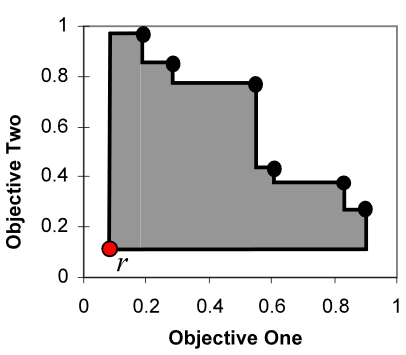
\includegraphics[scale=0.9]{hypervolume.png}
\caption{The figure shows how points from a Pareto front approximation and a reference point together form the region of objective space. The black dots are Pareto optimal solutions and the red dot is the reference point.}
\label{fig:hyperVolume}
\end{figure}

One important remark - the reference point must be consistent when evaluating approximations obtained by different learning algorithms. \\

\subsection{Experiment Structure.}

\subsubsection{Single-Policy Algorithms.}
Single-policy algorithms (Castelleti et al., 2002\nocite{castelletti2002reinforcement} or Gabor, Kalmar and Szepesvari, 1998\nocite{gabor1998multi}) are initialized with a set of preferences. After that the algorithm executes a number of learning episodes and hopefully it will learn the Q-function of the optimal policy for the specified preferences.

To illustrate the work of single policy algorithms consider the following example; A simple MDP was constructed, it consists only of three time steps. On every time step two actions are available - left and right. State transition is deterministic i.e. each action always leads to the same successor state. For more details refer to Figure~\ref{fig:decisionTree}.

\begin{figure}[ht]
\centering
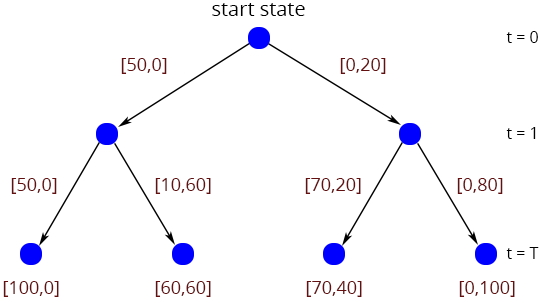
\includegraphics[scale=0.6]{decisionTree.png}
\caption{Blue circles represent states; Black arrows represent the actions. In every state left and right actions are available. State transition is deterministic and an action always leads to the same next state. Next to every arrow there is a vector of immediate rewards for choosing this action. The overall return starting from starting state is shown at the bottom of each branch.}
\label{fig:decisionTree}
\end{figure}

One can identify four different policies for this example MDP. Essentially, every branch of this tree is a unique policy with it's associated return.

It is possible to look at this problem from a different perspective - from the objective space. Figure~\ref{fig:exampleMDPFront} shows two dimensional objective space for the example MDP problem. Each blue dot corresponds to a unique policy and it's coordinates are exactly this policy's return. Overall there are four points in the objective space, one for each policy. One can notice that this four points together constitute the Pareto front for this problem. This is because the example MDP problem doesn't have dominated policies.

Consider any single-policy algorithm, for example one discussed in Castelleti et al. (2002)\nocite{castelletti2002reinforcement}. This algorithm requires a set of weights to be specified before the algorithm can start learning; Let $ \textbf{w} = \{0.4,0.6\} $ be this set of weights. Essentially, this algorithm is the multi-objective reinforcement learning adaptation of the linear-weighted average algorithm from general multi-objective optimization. Linear-weighted average algorithm will find which of the available solutions will maximize the dot product of the return vector and the weight vector.



\begin{figure}[ht]
\centering
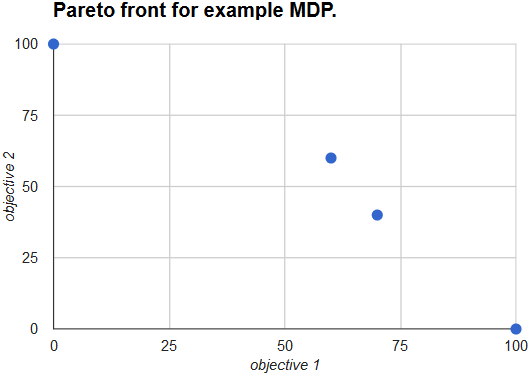
\includegraphics[scale=0.6]{exampleMDPFront.png}
\caption{Blue circles represent states; Black arrows represent the actions. In every state left and right actions are available. State transition is deterministic and an action always leads to the same next state. Next to every arrow there is a vector of immediate rewards for choosing this action. The overall return starting from starting state is shown at the bottom of each branch.}
\label{fig:exampleMDPFront}
\end{figure}

\subsection{Bechmarking Software.}
As was mentioned before a test problem in reinforcement learning is a dynamic software, which actively responds and changes according to the actions from an agent. The agent is also of dynamic nature and in the similar manner dynamically reacts to the changes in the test problem. This due to the inherent dynamic nature of the the agent-environment cycle. For example every test problem should have the means(function or method) to accept an action from the agent. As well as means(again function or a method) to pass information about state-transition and reward functions. \\

Even though test problems may have nothing in common in terms of realistic domains they represent, they still share those means of interaction with an agent or learning algorithm. Moreover in every problem the information that is passed between an agent and an environment is of very similar nature: the agent informs the environment about his preferred action, the environment notifies the agent about the consequences of that particular action. \\

For a long time nobody took advantage of that fact; Not only different programming techniques were used to implement the interaction between the agent and the environment but also different programming languages and different platforms were used. This created a natural level of complexity which prevented the exchange of learning algorithms and test problems. \\

Eventually Tanner and White (2009)\cite{tanner2009rl} created an open source software called RL-Glue. This software lays a foundation for empirical studies in reinforcement learning because it provides a necessary set of standards which allow to connect the test problems with the learning algorithms from different researchers without creation of this mundane connecting code. Essentially, RL-Glue, by introducing a set of standard functions , allows to plug-in agents, environments and experiments from different authors even created in different languages. \\

RL-Glue consists of the three main modules: an agent, an environment and an experiment. The agent is the module which encapsulates the learning algorithm. The environment is the module which encapsulates a particular test problem. The experiment is the program which serves as traditional main function and is responsible for running the agent through the environment and collecting all the data obtained by the agent. The experiment module is place where researcher controls how many episodes or how many trials should be performed by the agent. All the interaction between the modules is handled by a central server. \\
\begin{figure}[ht]
\vskip 0.2in
\centering
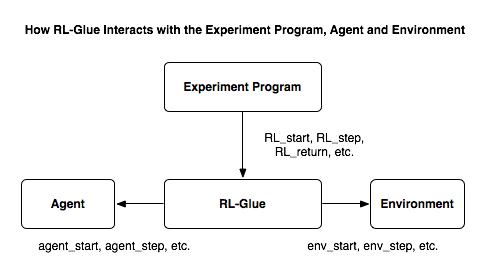
\includegraphics[scale=0.9]{glue.png}
\caption{The RL-Glue standard.}
\vskip -0.2in
\label{rlglue}
\end{figure}
The plug-in nature of the the RL-glue perfectly addresses three aspects of adequate methodology that were outlined before. Namely:

\begin{itemize}

\item The agent module encapsulates the learning algorithm to be evaluated. Each learning algorithm is a separate plug-in. Multiple number of the learning algorithms could be attached to the RL-glue simultaneously. This allows to evaluate multiple number of the algorithms simultaneously. A researcher just chooses which of the connected agents will be evaluated.

\item The environment module tackles aspect number two of the adequate methodology. Because the environment module is well-documented and well-standardized in terms of standard programming interfaces it allows to create standard test problems. This modules eliminates the need of connecting codes needed at the present moment. With plug-in architecture the researcher only needs to download a test problem and plug it into running RL-glue server without any connecting code.

\item The experiment module tackles aspect number three of the adequate methodology. The experiment module is the plug-in where the researcher chooses the particular test problem and the particular learning algorithms that will be evaluated against that test problem. The experiment module is also a place where all the statistics is gathered and analyzed. This is achieved by introducing a standard message protocol between the agent module and the experiment module. Using this message protocol the agents can send information about learned Q-functions and policies to the experiment module. This is also a place where different performance metrics are applied. Each performance metric is created as a library with external functions which encapsulates the inner routines. Such performance metrics are stored separately in the library files and also could be accessible to the public. For example Hypervolume performance metric will be introduced to RL-glue as a part of this thesis and will be available publicly. So if any other researcher wants to use it, the only job left to do is to download it and add to the existing libraries. When the performance metric library is downloaded and introduced to RL-glue it offers an interface of public functions which accept information obtained from the agent.

\end{itemize}

Originally, RL-Glue is a software for single objective reinforcement learning but it can be adapted to multi-objective(which is also a part of this thesis) by replacing scalar reward signal with vector-valued. \\

\subsection{Evaluation of the algorithms}

This research project aims to empirically evaluate algorithms belonging to two important classes: single policy algorithms and multi-policy algorithms. Though hypervolume performance metric will be used in both cases, there is important distinction between two approaches. The following two subsections will be devoted to explaining the methodology of empirical evaluation underlying both approaches.

\subsection{Single policy algorithms}

Multi-objective reinforcement learning covers a lot of real life problems. Which metric to use to evaluate different algorithms pretty much depends on the problem itself. Some of the problems have coherent objectives. For example consider a problem where one tries to maximize profit from introducing new technology but also needs to take into account the cost of introducing this new technology. These is a good example of the problem with coherent objectives. As was mentioned in literature review section single agent approaches are more suitable to this class of problems. This is also an example of the single policy problem where despite of the multiple number of objectives it is still perfectly acceptable to reduce number of objectives to a single optimization criteria and thus work to a single policy. Because all objectives are coherent no special metrics are required to perform the evaluation of the algorithms suitable for this task. One only need to pick a correct algorithms to compare like linear scalarisation. The weighted sum which is the core of the algorithm is itself a suitable metric to compare algorithms. \\

However, single agent algorithms are also suitable to problems where goals are isolated or even in conflict with each other. In this scenario it is no longer meaningful to use metric such as weighted sum because obviously objectives are of different nature. And obvious question arises - how to compare two multi-objective algorithms if their goals are not related to each other? Hypervolume metric is designed to evaluate the quality of the approximated Pareto front. But, unlike multi-policy algorithms, single-policy ones do not produce an approximation to the entire front, instead only a particular point of the front is learned by the algorithm. This particular point is basically predefined by the appropriate assignment of preferences to each of the objectives. So the traditional hypervolume metric is of no use. However, each of the points from the Pareto front could be found by varying preferences of the objectives. In this manner the approximation to the entire front could be found and hypervolume metric could be applied to evaluate the quality of the found Pareto front. This research project will employ this technique to evaluate single-policy algorithms. \\

The evaluation of two single-policy algorithms could be broken into stages:

\begin{itemize}

\item Create a range of preferences.

\item Use created range of preferences to find an approximation to the Pareto front of algorithm A.

\item Use created range of preferences to find an approximation to the Pareto front of algorithm B.

\item Use hypervolume to find which of the algorithms performed better.

\end{itemize}

\subsection{Multi-policy algorithms.}

In contrast to single policy algorithms, multi-policy algorithms try to find an approximation to the entire Pareto front. Examples of this class of algorithms are approaches proposed by (Shelton, \cite{Shelton2001}) and (Barrett, Narayanan, \cite{BarrettN2008}). To compare algorithms of this nature we need to use metric which will assess the quality of the approximated Pareto front. This is a perfect spot to apply hypervolume metric. \\

\begin{figure}[ht]
\vskip 0.2in
\centering
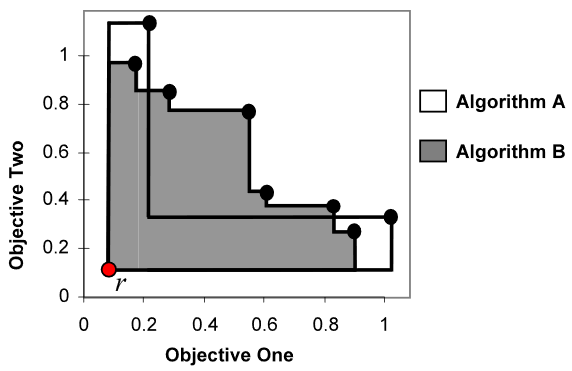
\includegraphics[scale=0.9]{2alghypervolume.png}
\caption{Example of using the hypervolume metric to evaluate two algorithms.}
\vskip -0.2in
\label{ParetoDominance}
\end{figure}

Contrary to single-policy algorithms, which at every moment of time are learning only a single point of the Pareto front, multi-policy algorithms at every moment have an approximation to the entire Pareto front. Thus it is possible to use hypervolume metric through the progress of the experiment and asses the quality of approximated front on the go. This metric should be calculated at specified time intervals. Thus it will be possible to evaluate the progress of the compared algorithms. This allows to identify which algorithms converge faster. \\

\begin{figure}[ht]
\vskip 0.2in
\centering
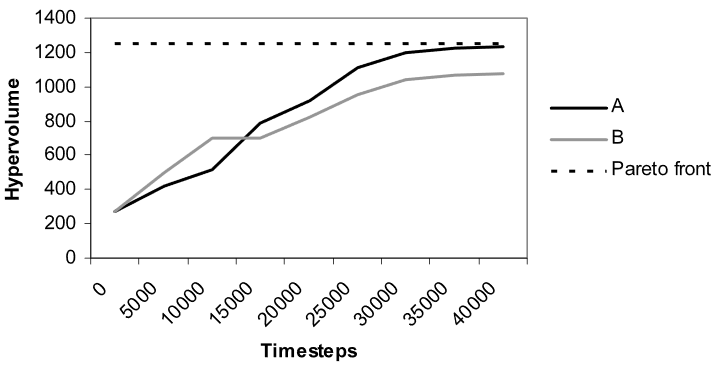
\includegraphics[scale=0.9]{2alghypervolumeovertime.png}
\caption{Example of calculating the hypervolume metric at specified time intervals to keep track of the progress of the algorithms.}
\label{ParetoDominance}
\end{figure}

As was mentioned in (Vamplew et al, \cite{VamplewDBID2011}) the exact time intervals should be determined with respect to a particular test problem due to varying difficulty and level of stochasticity of test problems. \\

\section{Benchmarks.}

Each benchmark or test problem is created to address a particular aspects of real-life problems. Thus a rich library of benchmarks should be available to adequately assess a learning algorithm. A suite of these benchmarks will allow to look at the learning from different point of views. Combined together, the benchmarks will allow to evaluate how different algorithms cope with following aspects of real-life problems:

\begin{itemize}

\item Multiple number of the objectives. To test which algorithms cope better when the number of objectives is increasing.

\item A range of benchmarks should be devoted to assess algorithms under stochasticity of reward and state transition functions.

\item One of the basic requirements is to create benchmarks with continuous state and action spaces.

\item Another important class of benchmarks is ones describing real-life problems with large dimensionality of state or action spaces that require the use of function approximation;

\item Problems with partially-observable states.

\item A mixture of episodic and continuing tasks;

\item Each real-life problem assumes existence of Pareto front of optimal solutions. This front exhibits a number of different characteristics. A number of benchmarks should be created to expose the learning algorithms to all possible characteristics of the Pareto front.

\end{itemize}

(Vamplew et al, \cite{VamplewDBID2011}) already introduced a number of benchmarks with known Pareto fronts. This greatly facilitates in the evaluation of the multi-objectives algorithms.

\subsection{Deep sea treasure.}
This test problem is a grid world consisting 10 rows and 11 columns as shown on figure 3.5. The grid represents undersea surface with multiple number of treasure spots available. One small remark - is that each treasure spot may have different treasure value. The agent is represented as a submarine. Four actions available to the agent - left, right, up, down. Each of the actions move submarine by one square in appropriate direction. First objective is pretty obvious - to find as much as possible of treasure. Second objective is to minimize time spent. \\
\begin{figure}[ht]
\vskip 0.2in
\centering
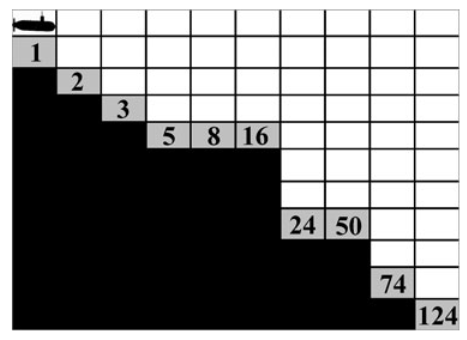
\includegraphics[scale=0.9]{dst.png}
\caption{Grid world for Deep Sea Treasure problem.}
\label{ParetoDominance}
\end{figure}

This problem comes with a known Pareto front which is shown in Figure 3.6. The form of the front is globally concave with number of local concavities.
\begin{figure}[ht]
\vskip 0.2in
\centering
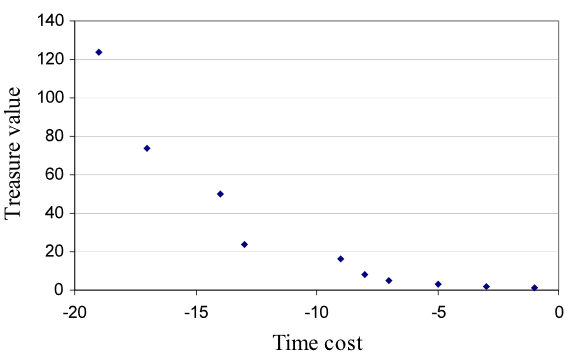
\includegraphics[scale=0.9]{dstPareto.png}
\caption{Pareto front for Deep Sea Treasure problem.}
\label{ParetoDominance}
\end{figure}

\subsection{MO-Puddleworld.}
This test problem represents 2 dimensional world with puddles located across the world as shown in Figure 3.7. Each episode agents starts at a random location and must reach the goal position(top-right corner) while avoiding the puddles. Four actions available to the agent - left, right, up, down. In this problem reward vector is represented as two penalties: first applied each time step until goal state is reached, second applied when the agent enters a puddle.
\begin{figure}[ht]
\vskip 0.2in
\centering
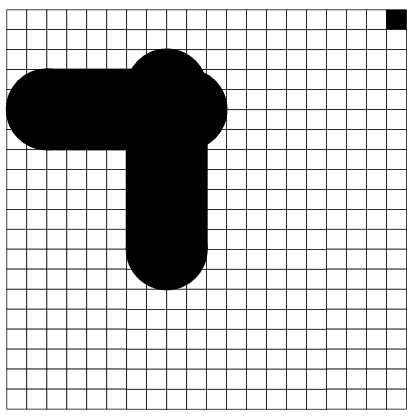
\includegraphics[scale=0.9]{pw.png}
\caption{Grid world for the Puddleworld problem.}
\label{ParetoDominance}
\end{figure}

The Puddleworld problem also comes with a known Pareto front which is shown in Figure 3.8.
\begin{figure}[ht]
\vskip 0.2in
\centering
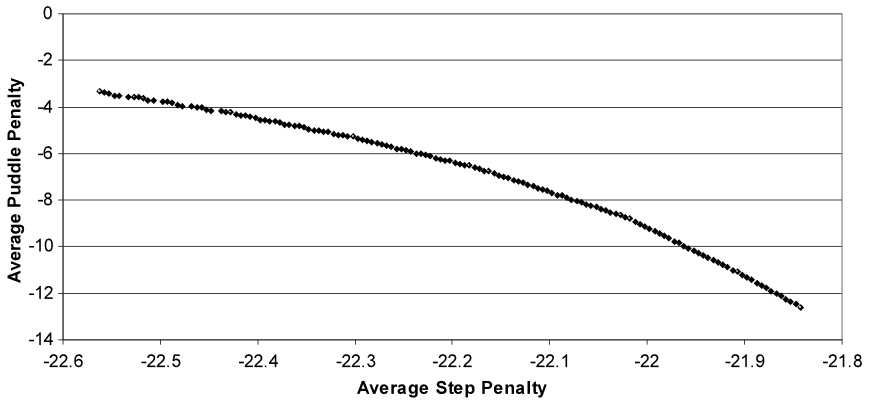
\includegraphics[scale=0.9]{pwParetoFront.png}
\caption{Pareto front for the Puddleworld problem.}
\label{ParetoDominance}
\end{figure}

From first inspection it is seen that the shape of the front is convex but at a closer inspection reveals a number of concavities and linearities. \\


\subsection{MO-Mountain Car.}
This test problem represents a valley with a car that must escape from the valley. But the car's engine is to weak to overcome the gravity so the car should climb left side of the valley with reverse acceleration to build enough potential energy to escape from the right side. Three actions available to the agent - full
throttle forward, full throttle backward, and zero throttle. A penalty of -1 is received on all states except the goal state. There are two additional penalties: -1 for earch reverse acceleration and -1 for each forward acceleration. So totally reward vector consists of three elements. \\

\subsection{Resource gathering.}
This test problem represents 2 dimensional grid world. Two types of resources are available for gathering - gold and gems. The goal of the agent is to gather either of both of the resources. Also there are locations where the hero can be attacked, the chance of being attacked is 10 percent. If the attack happens then the agent loses all gathered resources and returns to base. Four actions available to the agent - left, right, up, down. Each of the actions move the agent by one square in appropriate direction. The reward vector consists of three elements and is structured in the following way - [enemy, gold, gems]. \\
\begin{figure}[ht]
\vskip 0.2in
\centering
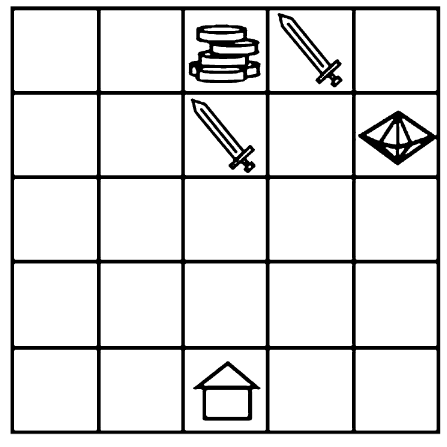
\includegraphics[scale=0.6]{rg.png}
\caption{Grid world for the Resource Gathering problem.}
\label{ParetoDominance}
\end{figure}

(Barrett, Narayanan, \cite{BarrettN2008}) used Convex Hull Value Iteration algorithm and found six optimal policies as shown on Figure 3.10.
\begin{figure}[ht]
\vskip 0.2in
\centering
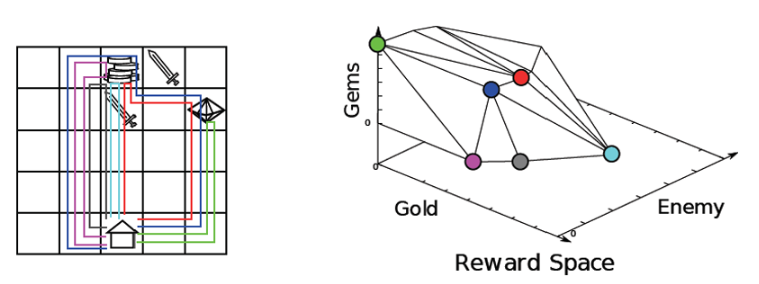
\includegraphics[scale=0.8]{rgpareto.png}
\caption{Optimal Policies for the Resource Gathering problem.}
\label{ParetoDominance}
\end{figure} 